\section{Related work}

\subsection{misc}


Lots of event-data studies. Also, complaints that models can't predict (\url{http://parusanalytics.com/eventdata/papers.dir/MPSA11.ICEWS.sequence2.1.pdf}).  We should develop a model that is both suggestive and predictive.  

this special issue: \url{http://onlinelibrary.wiley.com/doi/10.1111/jcom.2012.62.issue-2/issuetoc}

\subsection{\citep{mishra_enthusiasm_2014}}

\subsection{\citep{goldstone_cross-class_2011}}
If a protest draws support mainly from just one class or group (peasants, workers,
students, urban shopkeepers, professionals), the state can confront that group as a disruptive
force, and seek to unify elites from other sectors against that threat. However, if
protestors represent many different groups, it is much harder for the state to find allies
against them. Moreover, while a state can claim to be preserving society by acting
against isolated disruptive elements, it is far more difficult to maintain legitimacy when
acting against a broad cross-class coalition. Elites are more likely to desert the state, creating
crippling elite divisions, if protestors represent a broad spectrum of society. In
addition, a broad cross-class coalition facilitates further mobilization by creating ‘meganetworks’
linking prior, tightly-linked within-group networks to each other. The impact
of public media in favor of the protestors is also greater if media representation shows
protestors as representative of the whole society, rather than as one particular group
seeking partisan advantages for itself.

three successful revolutions in the Arab world in 2011, in Tunisia, Egypt, and Libya,
all demonstrate the crucial role of cross-class coalitions.

In short, what was just recently a remarkably tough coalition
capable of unseating a regime, even of conducting a civil war to do so, can become a pack
of feuding forces in the aftermath of successful revolt.
There are three ways that this fracturing of coalitions can play out – constructive opposition,
paralysis, or polarization.

It is too early to tell which outcome is most likely in the Arab revolts. It is still possible
that a future event


\subsection{isa from goldstone}

\url{https://isaconf.confex.com/isaconf/wc2014/webprogram/Paper40159.html}
When they began, there was hope that the Arab Revolutions of 2011 would be like the peaceful “velvet” or “color” revolutions in the USSR and Eastern Europe in 1989, or in the Ukraine in 2004.  Instead, with the possible exception of Tunisia, they have turned out to be more like true, classic revolutions with civil wars, counter-revolutions, high levels of violence, and extended periods of turmoil and sudden shifts in government.  There are a number of reasons for this difference, including (1) the greater youth of populations in the Arab revolutions; (2) the role of ideological contenders for power – Islamists – alongside the secular liberal revolutionaries; (3) the major interventions of outside powers; and (4) greater internal regional, ethnic and tribal divisions.


\subsection{\cite{goldstone_bringing_2013}}

    \begin{figure}[h]
        \centering
        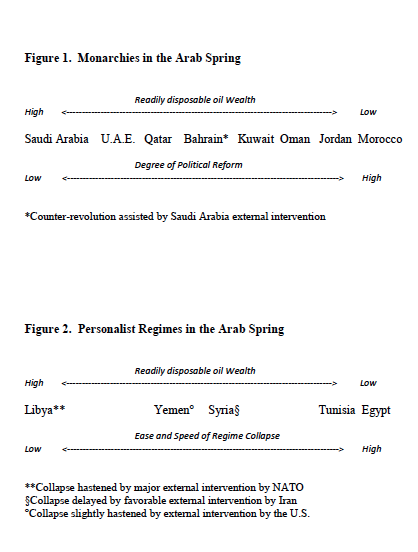
\includegraphics[width=.8\textwidth]{goldstone_2013_ssrn.png}
        \caption{\cite{goldstone_bringing_2013}}
        \label{fig:init_res}
    \end{figure}  

what resulted from this common foundation of unemployment, inequality, corruption, media links and protest differed enormously from country to country. In Tunisia, Egypt, and Yemen seemingly invulnerable autocrats who had ruled for decades surrendered power, stepping down or fleeing in the face of mounting nation-wide popular protests. In Libya and Syria similarly autocratic leaders instead mobilized for war and undertook an all-out military assault on their opponents; Libya’s failed but Syria’s regime has so far succeeded in holding on to power. In contrast, in Algeria, Iraq, Saudi Arabia and Bahrain protests fizzled or were quickly snuffled out. And in Morocco, Oman, Kuwait and Jordan monarchs turned to varying degrees of constitutional reform and working with elected parliaments; in these cases reforms appear to have brought peace by deflecting demands for revolt or revolution.

Three factors of regimes that indicate how they faired:
-personalist regimes (where a single individual – who may have begun as an elected leader, or head of a military or even party regime – takes control of the national government) are particularly vulnerable to revolutionary collapse in the event of widespread popular uprising
    -monarchies () were much more stable
    -Personalist regimes include the regimes of Saleh in Yemen, Ghaddafi in Libya, Assad in Syria, Ben Ali in Tunisia, and Mubarak in Egypt
    -Libya is the major outlier among the personalist regimes, with vast oil revenues forming the base of the economy and providing the regime with substantial resources.
    
-a number of regimes in the region rule major oil and gas producing states. As Michael Ross (2012) has argued, states that control revenues that are easily and secretly controlled, that do not require taxation, and that are large enough to give the state the ability to maintain a large cadre of elite supporters, institutions, and popular largesse have exceptional resilience against popular demands.
    -The oil-poor states (Morocco and Jordan) went the furthest in their reforms; the oil-rich states (Oman, Kuwait, Saudi Arabia) did the least
    
-a state’s position in the international states-system has major consequences for the possibilities of change.
    - Bahrain faced perhaps the most massive protests ever seen in an authoritarian regime, in proportion to its population. However, it received help from Saudi Arabia.

In sum, the single best key to where regimes in MENA have been overturned or faced massive rebellions is where personalist regimes have arisen. In contrast to the monarchies, which all have either survived with reforms or even become counter-revolutionary, the personalist regimes have all crumbled – with the exception of Syria, which is slowly succumbing to civil war and survives in large part because of a favorable balance of external intervention.
Among these regimes, the relative ease with which they were overthrown depended on the availability of oil revenues and the impact of international actions.


It has seemed odd to many that the Arab states not yet mentioned – Lebanon, the Palestinian Authority, Iraq, and Algeria – were hardly touched by the wave of protests that erupted in the Arab Spring.

This too can be explained by a focus on the state, rather than on the structural or populist reasons for protest. The countries where the Arab Spring had its impact were monarchies and personalist regimes

Egypt and Tunisia changed their regimes with relatively little violence. Yet their change has not gone as smoothly as hoped.

Yemen has had a relatively peaceful change of regime, but it has not had peace

The vast majority of revolutionary transitions took 5 years or more, with a median of 8 years

\cite{hussein_what_2013}

The early adopters were middle-class, educated, and underemployed, relatively leaderless, and technology-savvy youth.

Six "phases" to the revolution:
	preparation phase: involving activists’ use of digital media across time to build solidarity networks and identification of collective identities and goals
	ignition phase: involving symbolically powerful moments which ruling elites and regimes intentionally or lazily ignored, but which galvanized the public
	protest phase: by employing offline networks and digital technologies, small groups strategically organized on large numbers
	international buy-in phase: digital media networks extended the range of local coverage to international broadcast networks
	climax phase:  the regime maneuvered strategically or carelessly to appease public discontent through welfare packages or harsh repressive actions
	information warfare phase: various actors, state-based and from international civic advocacy networks, compete to shape the future of civil society

ICTS can also empower authoritarian security forces in improving their management and coercion capabilities.  It is wrongheaded
to construct a technologically deterministic theory of contemporary
democratization,


along with wealth, telecommunications and information policy can contribute to democratization (Norris 2001; Milner 2006; Howard and Mazaheri 2009). Many have hypothesized that increased Internet usage supports the growth of democratic institutions (Hogan 1999; Abbott 2001; George 2006).

Yet both democracies and dictatorships have fast-growing numbers of Internet
users, Internet hosts, mobile phones, and personal computers. Authoritarian
regimes may develop their digital communication infrastructure specifically to
extend state power (Kalathil and Boas 2003).

digital technologies (may) provide the entry points for young activists to explore democratic alternatives, an action landscape such as cyberspace that allows for political discourse and even direct interventions with state policy, and coordinating mechanisms that support synchronized social movements through marches, protests, and other forms of collective action (Kirsh 2001; Warschauer, El Said, and Zohry 2002; Abdulla 2005, 2007; Shapiro 2009).

it makes most sense to look for “conjoined causal conditions,” the set of multiple indicators that together provide a fulfilling narrative for understanding political outcomes. An examination of the political impacts of digital technologies should not assume positive or negative effects

Independent Variables used:
	Average Incomes Within Country
	Wealth Distribution (Gini)
	Levels of Unemployment
	Demographic Variables (pop. size, degree of urbanization, youth buldge)
	Censorship Sophistication (we created an index combining the OpenNet Initiative’s monitoring of countries that had instituted no filtering, or a range of selective, substantial, and pervasive filtering on content for political, social, security reasons or used automated tools to do s)
	Fuel-dependent Economy (countries’ level of oil production and its share in the global oil resources available)

Dependent variables
	Regime Fragility - Full membership in the set of fragile Arab Spring countries was given to the countries where street turnout was surprisingly large, attendance was consistently high over several days, domestic media attention unusually interested, and protests took place in an unexpected number of diverse locations. Lower scores went to cases where protest turnout was small, concentrated in only a few locations, or protesters themselves were quickly dissuaded.
	Social Movement Success 

Results:
First, not being a country where the national economy is dependent on fuel exports is a consistent ingredient in all the recipes of social movement success. Second, widespread use of mobile phone technologies was less important for the success of social movements than Internet use. However, the latter does appear as a key ingredient in two causal recipes. Therefore, having a mobile-enabled population is useful, particularly when protests have been ignited. But more than access to mobile technologies, having a long-term Internet-enabled civil society appears in all recipes.

Discussion
For scholars of social movements and collective action, there are several
interesting aspects of the Arab Spring: the distributed leadership of protest
organizers, the core groups of elite publics (literate, middle class, youth, women,
and technocrats) that were relatively quick in joining them, and the important
role that international news organizations played in giving them the global exposure
to help stave off overtly violent reactions from security forces.

Digital media had a causal role in the
Arab Spring by providing the very infrastructure that created deep communication
ties and organizational capacity in groups of activists before the major protests
took plac

For the most part, it was physical
intimidation that discouraged activists from communicating about their political
activity on Facebook

A peripheral
counting of media use and digital diffusion levels reveals that the countries
experiencing the most dramatic changes had low overall percentages of social
media use (Mourtada and Salem 2011). But limiting the analysis to aggregate
indicators precludes the possibility of telling a more complex, causal story. Moreover,
if there is anything to the analytical frame of networks, the use of important
media by a few important nodes of users could be exceptionally
consequential. This is why, to unpack the complexities of the Arab Spring, we
must employ analytic approaches that make possible the examination of complex
social systems that constitute the overall aggregate of state-based cases.


.... summary ....

social media helped democratic ideas spread across borders, through informal networks of families, friends, and interested onlookers.

The intensity of political conversations that took place preceding major street protests supports the idea that virtual networks materialized before street protest networks.

Facebook pages and Twitter conversations were essential for designing and trying out new strategies as events took place on the ground.




\subsection{\cite{goldstone_bringing_2013}}

    \begin{figure}[h]
        \centering
        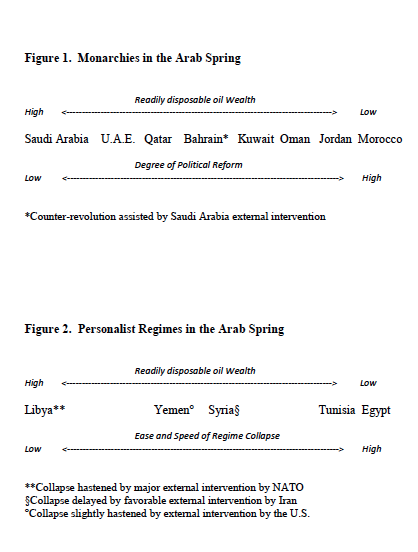
\includegraphics[width=.8\textwidth]{goldstone_2013_ssrn.png}
        \caption{\cite{goldstone_bringing_2013}}
        \label{fig:init_res}
    \end{figure}  

In Tunisia, Egypt, and Yemen seemingly invulnerable autocrats who had ruled for decades surrendered power, stepping down or fleeing in the face of mounting nation-wide popular protests. 

In Libya and Syria similarly autocratic leaders instead mobilized for war and undertook an all-out military assault on their opponents; Libya’s failed but Syria’s regime has so far succeeded in holding on to power. 

In contrast, in Algeria, Iraq, Saudi Arabia and Bahrain protests fizzled or were quickly snuffled out. 

And in Morocco, Oman, Kuwait and Jordan monarchs turned to varying degrees of constitutional reform and working with elected parliaments; in these cases reforms appear to have brought peace by deflecting demands for revolt or revolution.

Three factors of regimes that indicate how they faired:
-personalist regimes (where a single individual – who may have begun as an elected leader, or head of a military or even party regime – takes control of the national government) are particularly vulnerable to revolutionary collapse in the event of widespread popular uprising
    -monarchies () were much more stable
    
    parties are used as vehicles to push specific people through 
    
    -Personalist regimes include the regimes of Saleh in Yemen, Ghaddafi in Libya, Assad in Syria, Ben Ali in Tunisia, and Mubarak in Egypt
    -Libya is the major outlier among the personalist regimes, with vast oil revenues forming the base of the economy and providing the regime with substantial resources.
    
-a number of regimes in the region rule major oil and gas producing states. As Michael Ross (2012) has argued, states that control revenues that are easily and secretly controlled, that do not require taxation, and that are large enough to give the state the ability to maintain a large cadre of elite supporters, institutions, and popular largesse have exceptional resilience against popular demands.
    -The oil-poor states (Morocco and Jordan) went the furthest in their reforms; the oil-rich states (Oman, Kuwait, Saudi Arabia) did the least
    
-a state’s position in the international states-system has major consequences for the possibilities of change.
    - Bahrain faced perhaps the most massive protests ever seen in an authoritarian regime, in proportion to its population. However, it received help from Saudi Arabia.

In sum, the single best key to where regimes in MENA have been overturned or faced massive rebellions is where personalist regimes have arisen. In contrast to the monarchies, which all have either survived with reforms or even become counter-revolutionary, the personalist regimes have all crumbled – with the exception of Syria, which is slowly succumbing to civil war and survives in large part because of a favorable balance of external intervention.
Among these regimes, the relative ease with which they were overthrown depended on the availability of oil revenues and the impact of international actions.


It has seemed odd to many that the Arab states not yet mentioned – Lebanon, the Palestinian Authority, Iraq, and Algeria – were hardly touched by the wave of protests that erupted in the Arab Spring.

This too can be explained by a focus on the state, rather than on the structural or populist reasons for protest. The countries where the Arab Spring had its impact were monarchies and personalist regimes

Egypt and Tunisia changed their regimes with relatively little violence. Yet their change has not gone as smoothly as hoped.

Yemen has had a relatively peaceful change of regime, but it has not had peace

The vast majority of revolutionary transitions took 5 years or more, with a median of 8 years



Six "phases" to the revolution:
	preparation phase: involving activists’ use of digital media across time to build solidarity networks and identification of collective identities and goals
	ignition phase: involving symbolically powerful moments which ruling elites and regimes intentionally or lazily ignored, but which galvanized the public
	protest phase: by employing offline networks and digital technologies, small groups strategically organized on large numbers
	international buy-in phase: digital media networks extended the range of local coverage to international broadcast networks
	climax phase:  the regime maneuvered strategically or carelessly to appease public discontent through welfare packages or harsh repressive actions
	information warfare phase: various actors, state-based and from international civic advocacy networks, compete to shape the future of civil society
	

regime 
class-spread
Average Incomes Within Country
Wealth Distribution (Gini)
Levels of Unemployment
Demographic Variables (pop. size, degree of urbanization, youth buldge)
Censorship Sophistication 
Fuel-dependent Economy 

Regime Fragility 	
Social Movement Success 

black-out of media vs not black out media 
religious freedom indices

Twitter
News 
international network position
Ethnic diversity / group indicators

Twitter and news as independent or representative of?


